\documentclass{article}
\usepackage[utf8]{inputenc}

\title{TT3010 - Audio technology and room acoustics. \newline Exercise 4 - Loudspeakers in rooms \newline Solutions}
\author{Jan Arne Bosnes}
\date{\today}

\usepackage{natbib}
\usepackage{graphicx}
\usepackage{float}
\usepackage{gensymb}

\begin{document}

\maketitle

\section*{Tasks}

\subsection*{1}

Remember that the speed of sound $c$,  the frequency $f$ and wavelength $\lambda$. have the following relation.

\begin{equation}
    c=f \lambda
\end{equation}

If we rearrange the expression and insert the diameter $d$, of the woofer, we get the frequency:

\begin{equation}
    f_{woofer}=\frac{c}{d_{woofer}} \approx 900 \ Hz
\end{equation}

The same thing can be done for the tweeter.

\begin{equation}
    f_{tweeter} = \frac{c}{d_{tweeter}} \approx 6860 \ Hz
\end{equation}

\subsection*{2}

The acoustic power output $W_{Ac}$ of the sound system is equal to the product of the electrical input power $W_{ele}$ and the efficiency of the sound system $\eta$. Then $W_{Ac}=\eta W_{ele}=0.5$ kW.

Now we can express the sound power level radiated by the speaker in terms of decibel using the following expression.

\begin{equation}
    L_W = 10 \log{\frac{W_{Ac}}{W_0}}
\end{equation}
where $W_0 = 10^{-12}$ W. This gives us a sound power level of $L_W \approx 147 $ dB.

We can now calculate the free field sound pressure level at 90 m and with a $Q$-factor that is 4.

\begin{equation}
    L_p = L_w + 10 \log{\frac{Q}{4 \pi r^2}}
\end{equation}

This gives $L_p \approx 103 $ dB.


\subsection*{3}

For an octave band, the upper cut-off frequency is twice the lower cut-off frequency. Therefore, if $f_{up}$ and $f_{low}$ represent the upper and lower cut-off frequencies,

\begin{equation}
    f_{up} = 2 f_{low}
\end{equation}

Furthermore, the center frequency of an octave filter is $f_{center}=\sqrt{f_{up}f_{low}}$.

We can then substitute $2f_{low}$ in the equation to get $$f_{center}=\sqrt{2f_{low}f_{low}}=\sqrt{2}f_{low}$$

Knowing this, we can express $f_{low}$ in terms of $f_{center}$.

\begin{equation}
    f_{low} = \frac{f_{center}}{\sqrt{2}}
\end{equation}

So, the lower cut-off frequency will be $f_{low}=\frac{500}{\sqrt{2}} \approx 354 \ Hz$.
and the upper cut-off frequency will then be $f_{up}=2 f_{low} \approx 707 \ Hz$


\subsection*{4}

Oscillations, or howling, due to acoustic feedback will occur if the distance between the microphone and the loudspeaker is equal to the wavelength of sound or a integer multiple thereof (and if the gain is high enough). Thus, the condition for oscillation due to acoustic feedback can be expressed as $n\lambda = d$, where $n$ is an integer, $\lambda$ is the wavelength and $d$ is the distance between microphone and loudspeaker.

Substituting $\lambda$ with $\frac{c}{f}$, we get the following expression for the frequencies that experience maximally strong acoustic feedback.

\begin{equation}
    f = \frac{n \cdot c}{d}
\end{equation}

The minimum frequency $f_{min}$ can be found by inserting $n$ = 1. $$f_{min}= \frac{1 \cdot 343}{5} = 69\ {\rm Hz}$$ 
which is the lowest frequency for which oscillation could take place. If one inserts positive integers for n (e.g 1,2,3,4,...), one will find the harmonics of $f_{min}$, which is the frequencies where you might experience oscillation due to (positive) feedback.

\subsection*{5}

When speaking at a normal conversational level, an average speaker emits about $10^-5$ W sound power. If there are $n$ speakers, each radiating a power $P$, then the time needed to generate an amount of energy $E$ can be calculated realizing that energy is equal to the product of power and time.

\begin{equation}
    E \cdot P \cdot t \rightarrow t=\frac{E}{nP}
\end{equation}

It takes around 1050 J energy to increase the temperature of water (tea) by $1\degree$C. Consider tea to be at room temperature, 25 $\degree$C, which is to be raised to 100 $\degree$C. The total energy  needed to boil a cup of tea, will then be $E = 1050 \cdot 75 \ {\rm J} \approx 7.875 \times 10^4$ J. The time to generate this amount of energy is then

\begin{equation}
    t =  \frac{E}{nP} = \frac{7.875 \times 10^4}{50 \cdot 10^-5}1.575 \times 10^8 \ {\rm s} = \approx 5  \ {\rm years}
\end{equation}
So, the statement is valid.

\subsection*{6}

\subsubsection*{a}

We can use the $x$-axis $r/\sqrt{Q}$ to find the related difference $L_p-L_W$.

\begin{equation}
    \frac{r_5}{\sqrt{Q}}= \frac{5}{\sqrt{2}} \approx 3.5 \rightarrow L_p - L_W \approx -18 {\rm dB} \rightarrow L_p = 80 - 18 = 62 {\rm dB}
\end{equation}

\begin{equation}
    \frac{r_{15}}{\sqrt{Q}}= \frac{15}{\sqrt{2}} \approx 10.6 \rightarrow L_p - L_W \approx -21 {\rm dB} \rightarrow L_p = 80 - 21 = 59 {\rm dB}
\end{equation}

\begin{figure}[H]
    \centering
    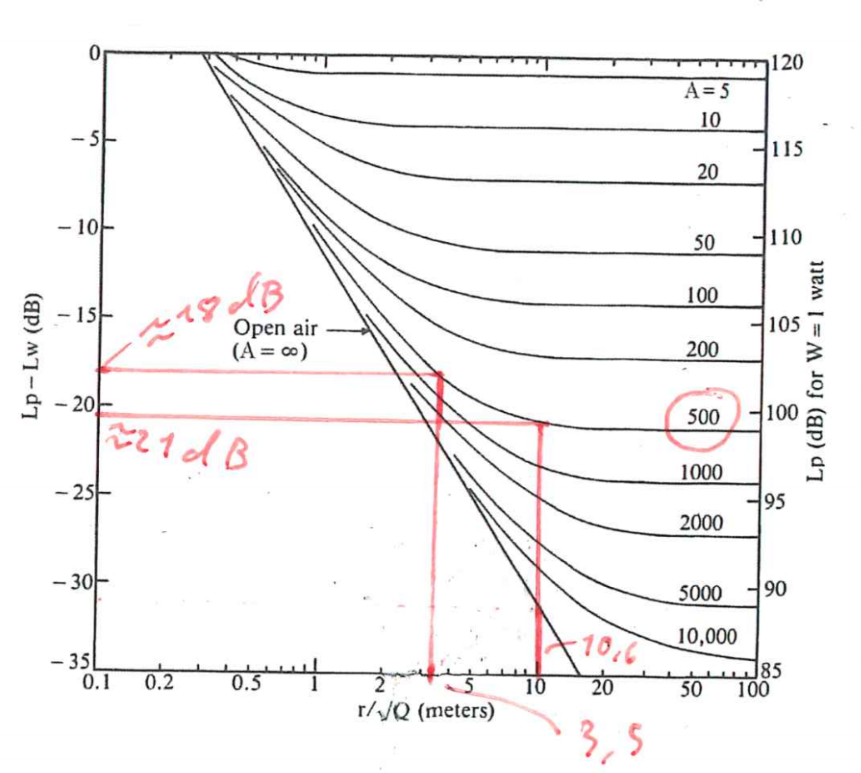
\includegraphics{figures/oving4_1_solution.png}
    \caption{Illustration for task 6a}
    \label{fig:my_label}
\end{figure}

\subsubsection*{b}

\begin{equation}
        L_{p,5} = L_W + 10\log(\frac{Q}{4 \pi r_5^2} + \frac{4}{A}) \approx 60.6 {\rm dB}
\end{equation}

\begin{equation}
        L_{p,15} = L_W + 10\log(\frac{Q}{4 \pi r_5^2} + \frac{4}{A}) \approx 59.4 {\rm dB}
\end{equation}



%\bibliographystyle{plain}
%\bibliography{references}
\end{document}
